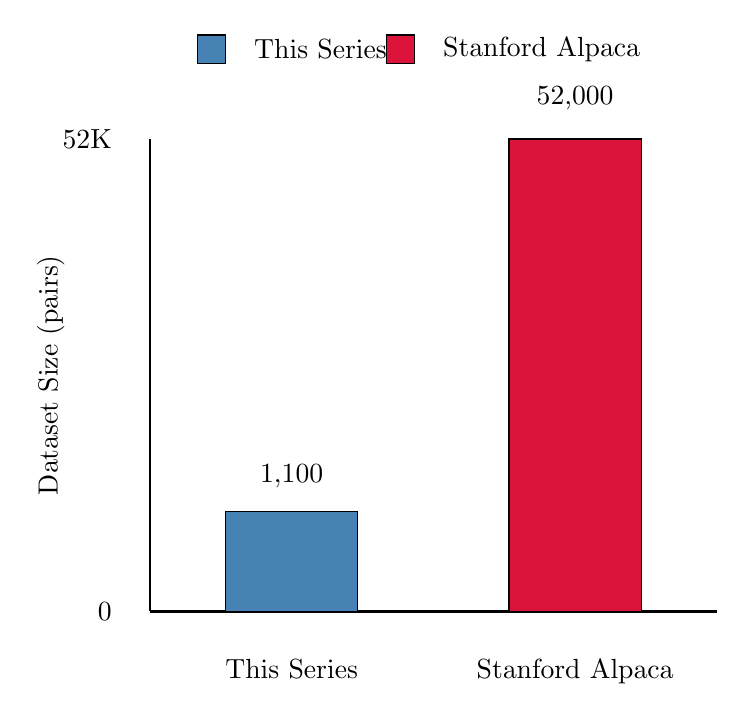
\begin{tikzpicture}[scale=1.2]
  % Define colors
  \definecolor{thisseriescolor}{RGB}{70, 130, 180}
  \definecolor{alpacacolor}{RGB}{220, 20, 60}
  
  % Y-axis
  \draw[thick] (0,0) -- (0,5);
  \draw[thick] (0,0) -- (6,0);
  
  % Y-axis labels
  \node[left] at (-0.3, 0) {0};
  \node[left] at (-0.3, 5) {52K};
  \node[left, rotate=90, anchor=south] at (-0.8, 2.5) {Dataset Size (pairs)};
  
  % X-axis labels
  \node[below] at (1.5, -0.4) {This Series};
  \node[below] at (4.5, -0.4) {Stanford Alpaca};
  
  % Bar for This Series (1,100 pairs)
  \draw[fill=thisseriescolor] (0.8, 0) rectangle (2.2, 1.06);
  \node[above] at (1.5, 1.2) {1,100};
  
  % Bar for Stanford Alpaca (52,000 pairs)
  \draw[fill=alpacacolor] (3.8, 0) rectangle (5.2, 5);
  \node[above] at (4.5, 5.2) {52,000};
  
  % Legend
  \draw[fill=thisseriescolor] (0.5, 5.8) rectangle (0.8, 6.1);
  \node[right] at (1, 5.95) {This Series};
  
  \draw[fill=alpacacolor] (2.5, 5.8) rectangle (2.8, 6.1);
  \node[right] at (3, 5.95) {Stanford Alpaca};
\end{tikzpicture}